\newcommand{\chapter}[2][]{
	\newcommand{\chapname}{#2}
	\begin{flushleft}
		\begin{minipage}[t]{\linewidth}
			
\includegraphics[height=1cm]{hdht-logo.png}
			\hspace{0pt}	
			\sffamily\bfseries\large Bài  18.
			\begin{flushleft}
				\LARGE\bfseries #1
			\end{flushleft}
		\end{minipage}
	\end{flushleft}
	\vspace{1cm}
	\normalfont\normalsize
}
\chapter[Một số loại lực thường gặp trong thực tiễn:\\ Lực ma sát, lực cản và lực nâng trong chất lưu]{Một số loại lực thường gặp trong thực tiễn: \\Lực ma sát, lực cản và lực nâng trong chất lưu}
\section{Lý thuyết}

\subsection{Lực ma sát trượt}
\subsubsection{Định nghĩa}
Lực ma sát trượt xuất hiện ở mặt tiếp xúc khi một vật trượt trên một bề mặt và cản trở lại chuyển động trượt của vật đó.
\begin{center}
	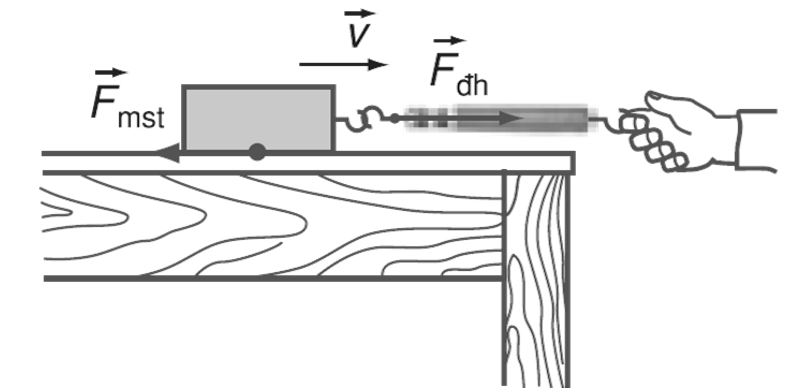
\includegraphics[scale=0.35]{../figs/VN10-PH-15-L-012-1-V2-01.JPG}
\end{center}
\subsubsection{Đặc điểm}
\begin{itemize}
	\item Phương: tiếp tuyến với mặt tiếp xúc giữa 2 vật trượt.
	\item Chiều: ngược chiều với vận tốc tương đối của vật ấy đối với vật kia.
	\item Độ lớn:
		\begin{itemize}
			\item không phụ thuộc vào diện tích tiếp xúc và tốc độ của vật.
			\item tỉ lệ với độ lớn của áp lực.
			\item phụ thuộc vào vật liệu và tình trạng của hai mặt tiếp xúc.
		\end{itemize}
	\item Biểu thức 
	\begin{equation*}
		F_{\text{mst}} = \mu_{\text{t}} \cdot N,
	\end{equation*}
	trong đó:
	
	+ $\mu_{\text{t}}$ là hệ số ma sát trượt, nó phụ thuộc vào bản chất của hai mặt tiếp xúc và các điều kiện trên bề mặt (không có đơn vị),
	
	+ $N$ là áp lực của vật lên mặt tiếp xúc.
\end{itemize}
\subsubsection{Vai trò}
\begin{itemize}
	\item Ma sát trượt có ích trong việc mài dũa, thắng xe …
	\item Ma sát trượt có hại trong các ổ trục trượt, mài mòn xilanh, pittông xe… Để giảm ma sát trượt, người ta bôi trơn các chi tiết bằng dầu mỡ công nghiệp.
\end{itemize}
\subsection{Lực ma sát lăn}
\begin{itemize}
	\item Lực ma sát lăn xuất hiện ở mặt tiếp xúc khi một vật lăn trên một bề mặt và cản trở lại chuyển động lăn của vật đó.
	\item Lực ma sát lăn có các đặc điểm giống như lực ma sát trượt nhưng hệ số ma sát lăn nhỏ hơn rất nhiều lần (hàng chục lần) hệ số ma sát trượt.
	\item Trong trường hợp lực ma sát trượt có hại, cần phải giảm thì người ta dùng con lăn hay ổ bi đặt xen vào giữa hai mặt tiếp xúc để giảm tổn hại vì ma sát.
\end{itemize}
\begin{center}
	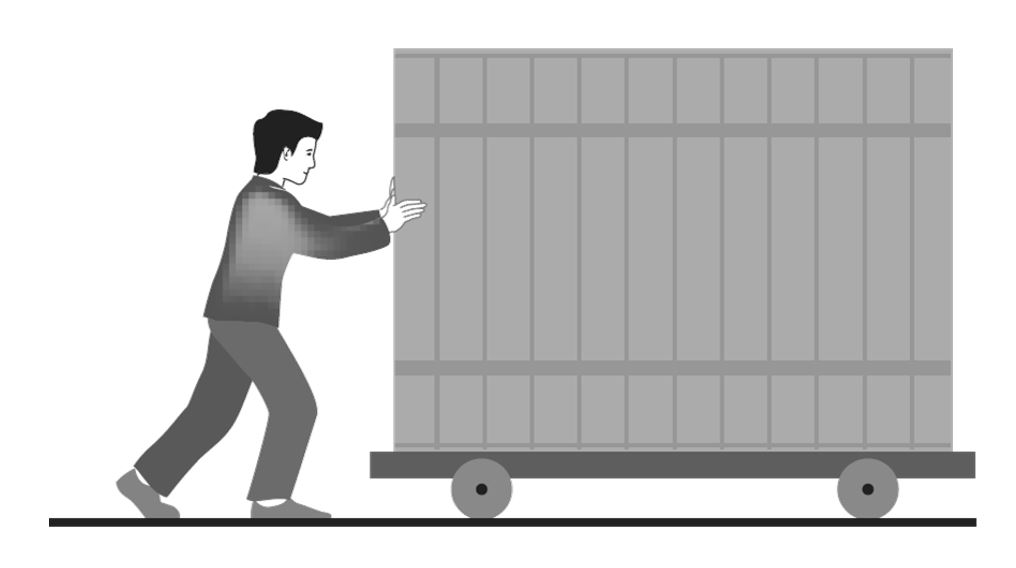
\includegraphics[scale=0.35]{../figs/VN10-PH-15-L-012-1-V2-02.JPG}
\end{center}
\subsection{Lực ma sát nghỉ}
\subsubsection{Định nghĩa}
Lực ma sát nghỉ xuất hiện ở mặt tiếp xúc khi một vật nằm yên trên bề mặt
vật khác và có xu hướng chuyển động dưới tác dụng của ngoại lực.
\begin{center}
	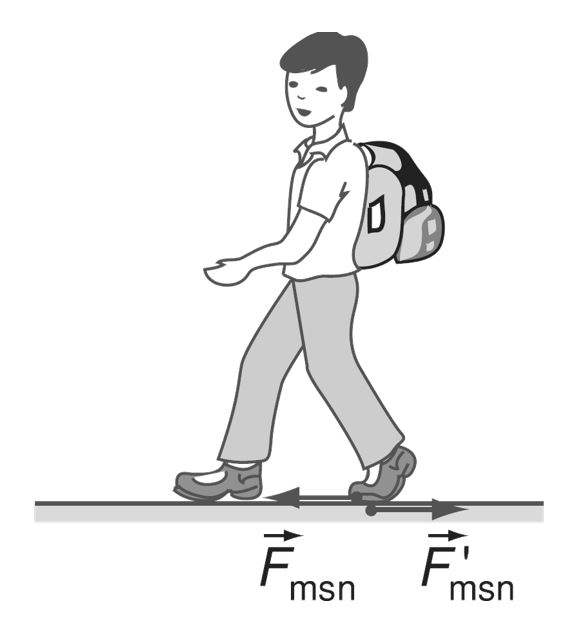
\includegraphics[scale=0.35]{../figs/VN10-PH-15-L-012-1-V2-03.JPG}
\end{center}
\subsubsection{Đặc điểm}
\begin{itemize}
	\item Lực ma sát nghỉ có điểm đặt trên vật, có hướng ngược với hướng của ngoại lực tác dụng song song với mặt tiếp xúc, có độ lớn bằng độ lớn ngoại lực tác dụng vào vật khi vật còn chưa chuyển động.
	\item Khi lực tác dụng song song với mặt tiếp xúc lớn hơn một giá trị nào đó thì vật sẽ trượt. Tuy nhiên lực ma sát nghỉ cực đại lớn hơn ma sát trượt.
\end{itemize}
\subsubsection{Vai trò}
\begin{itemize}
	\item Giúp ta cầm nắm được các vật, giữ vật ở yên tại vị trí đã định, dây cua roa truyền được chuyển động giữa các bánh xe, băng chuyền vận chuyển được người hoặc vật từ nơi này đến nơi khác...
	\item Đóng vai trò lực phát động, giúp sinh vật, xe cộ di chuyển được.
	\item Trong những trường hợp ma sát có lợi, người ta tìm cách tăng tính nhám của các mặt tiếp xúc và tăng áp lực lên mặt tiếp xúc, chẳng hạn thêm các rãnh trên đế giày, bánh xe để tăng ma sát.
\end{itemize}
\subsection{Các lực tác động lên vật chuyển động trên mặt phẳng ngang có ma sát}
	\begin{center}
	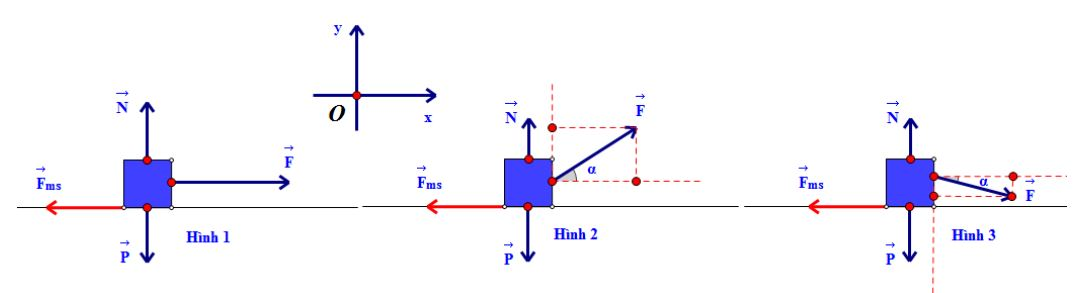
\includegraphics[scale=0.5]{../figs/VN10-PH-15-A-005-3-V2-01.JPG}
\end{center} 
\manatip{
	\begin{itemize}
		\item 
		
		Cách làm chung cho bài toán này thường theo hai bước 
		\begin{itemize}
			\item chiếu phương trình định luật II Newton lên trục O$y$ để tìm biểu thức của phản lực, từ đó suy ra công thức của lực ma sát
			\item chiếu phương trình định luật II Newton lên trục O$x$ để giải đại lượng cần tìm (gia tốc hoặc lực chưa biết). 
		\end{itemize}  
		
		\item 	Vật trượt đều thì gia tốc bằng 0.
\end{itemize}}
\begin{itemize}
	\item Biểu thức định luật II Newton tổng quát cho vật trượt ngang có ma sát
	\begin{equation*}
		\vec{F} +\vec{P} + \vec{F}_{\text{ms}} + \vec{N} =m\vec{a},
	\end{equation*}
	trong đó:
		\begin{itemize}
			\item $F$ là lực phát động,
			\item $P$ là trọng lực,
			\item $F_{\text{ms}}$ là lực ma sát, 
			\item $N$ là phản lực của mặt phẳng ngang có độ lớn bằng áp lực.
		\end{itemize}

	\item Hình 1
	
	+ Chiếu lên O$y$: 
	\begin{equation*}
		N-P =0  \Rightarrow N = P = mg \Rightarrow F_{\text{ms}} = \mu N = \mu \cdot mg.
	\end{equation*}
	+ Chiếu lên O$x$: 
	\begin{equation*}
		F-F_{\text{ms}} = ma \Rightarrow F - \mu mg =ma
	\end{equation*}
	\item Hình 2
	
	+ Chiếu lên O$y$: 
	\begin{equation*}
		N-P + F\sin \alpha =0  \Rightarrow N = P - F\sin \alpha = mg - F\sin \alpha,
	\end{equation*}
	\begin{equation*}
		\Rightarrow F_{\text{ms}} = \mu N = \mu (mg - F\sin \alpha).
	\end{equation*}
	+ Chiếu lên O$x$: 
	\begin{equation*}
		F\cos \alpha-F_{\text{ms}} = ma \Rightarrow F\cos \alpha - \mu (mg-F\sin \alpha) =ma
	\end{equation*}
	
	\item Hình 3
	
	+ Chiếu lên O$y$: 
	\begin{equation*}
		N-P - F\sin \alpha =0  \Rightarrow N = P + F\sin \alpha = mg + F\sin \alpha,
	\end{equation*}
	\begin{equation*}
		\Rightarrow F_{\text{ms}} = \mu N = \mu (mg + F\sin \alpha).
	\end{equation*}

	+ Chiếu lên O$x$: 
	\begin{equation*}
		F\cos \alpha-F_{\text{ms}} = ma \Rightarrow F\cos \alpha - \mu (mg+F\sin \alpha) =ma
	\end{equation*}
\end{itemize}

\subsection{Lực cản của chất lưu}
Chất lưu (flow) là những chất có thể chuyển động thành dòng. Ví dụ: chất lỏng, chất khí.
Mọi vật chuyển động trong chất lưu luôn chịu tác dụng bởi lực cản của chất lưu. Lực này ngược hướng chuyển động và cản trở chuyển động của vật.
\begin{center}
	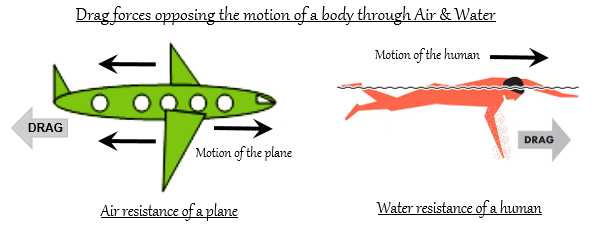
\includegraphics[scale=0.8]{G10-16-1.png}
\end{center}
Lực cản của chất lưu phụ thuộc vào hình dạng (khí động học) và tốc độ chuyển động của vật.
\subsection{Lực nâng của chất lưu}
Khi chuyển động trong chất lưu, ngoài lực cản thì vật còn chịu tác dụng của lực nâng.
\begin{center}
	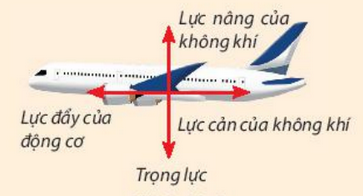
\includegraphics[scale=0.8]{G10-16-2.png}
\end{center}
Thông thường, ta hay đề cập đến một trường hợp riêng của lực nâng trong chất lưu, gọi là lực đẩy Ác-si-mét (Archimède), là lực hướng ngược chiều với trọng lực, có độ lớn theo công thức
$$F_\text{A} = \rho g V,$$
trong đó:
\begin{itemize}
	\item $F_\text{A}$ là lực đẩy Ác-si-mét (N);
	\item $\rho$ là khối lượng riêng của chất lưu ($\SI{}{kg/m^3}$);
	\item $V$ là phần thể tích chất lưu bị vật chiếm chỗ ($\SI{}{m^3}$).
\end{itemize}
\section{Mục tiêu bài học - Ví dụ minh họa}
\begin{dang}{Ghi nhớ khái niệm các loại lực ma sát}
	\viduii{1}{Hệ số ma sát trượt
		\begin{mcq}
			\item tỉ lệ thuận với lực ma sát trượt và tỉ lệ nghịch với áp lực. 
			\item phụ thuộc diện tích tiếp xúc và tốc độ của vật.
			\item phụ thuộc vào vật liệu và tình trạng của mặt tiếp xúc. 
			\item phụ thuộc vào áp lực.
		\end{mcq}
	}
	{	\begin{center}
			\textbf{Hướng dẫn giải}
		\end{center}
		
		Hệ số ma sát trượt phụ thuộc vào vật liệu và tình trạng của mặt tiếp xúc   
		
		\textbf{Đáp án: C}.
	}
	\viduii{1}{Chiều của lực ma sát nghỉ
		\begin{mcq}
			\item  Ngược chiều với vận tốc của vật.
			\item  Ngược chiều với gia tốc của vật.
			\item  Ngược chiều với thành phần ngoại lực song song với mặt tiếp xúc.
			\item  Vuông góc với mặt tiếp xúc.
		\end{mcq}
	}
	{	\begin{center}
			\textbf{Hướng dẫn giải}
		\end{center}
		
		Chiều của lực ma sát nghỉ ngược chiều với thành phần ngoại lực song song với mặt tiếp xúc.
		
		\textbf{Đáp án: C}.
	}
	\viduii{1}{Phát biểu nào sau đây là đúng khi nói về ma sát
		\begin{mcq}
			\item Lực ma sát lăn cản trở chuyển động của vật này trượt trên vật khác.
			\item Khi vật chuyển động chậm dần, lực ma sát nhỏ hơn lực đẩy.
			\item Lực ma sát lăn nhỏ hơn lực ma sát trượt.
			\item Khi vật chuyển động nhanh dần, lực ma sát lớn hơn lực đẩy.
		\end{mcq}
	}
	{	\begin{center}
			\textbf{Hướng dẫn giải}
		\end{center}
		
		A - sai vì: lực ma sát lăn cản trở chuyển động của vật này lăn trên vật khác
		
		B - sai vì: khi vật chuyển động chậm dần, lực ma sát lớn hơn lực đẩy
		
		C - đúng
		
		D - sai vì: khi vật chuyển động nhanh dần, lực ma sát nhỏ hơn lực đẩy
		
		\textbf{Đáp án: C}.
	}
\end{dang}
\begin{dang}{Tính lực và các đại lượng\\ trong công thức lực ma sát trượt}
	\viduii{2}{Một ô tô khối lượng 1,5 tấn chuyển động thẳng đều trên đường. Hệ số ma sát lăn giữa bánh xe và mặt đường là 0,08. Tính lực làm cản trở chuyển động của xe trên mặt đường (bỏ qua lực cản không khí).
	}
	{	\begin{center}
			\textbf{Hướng dẫn giải}
		\end{center}
		 \manatip{Trong trường hợp xe chuyển động do lực đẩy của động cơ, ta xem như lực này có phương song song với mặt đất.}
		
		Lực đẩy song song với mặt ngang, nên phản lực có độ lớn bằng với trọng lực. Lực làm cản trở chuyển động của xe trên mặt đường là lực ma sát
		\begin{equation*}
			F_{\text{ms}} =\mu N = \mu  mg =\SI{0.08}{}\cdot(\SI{1.5e3}{\kilogram})\cdot\SI{9.81}{\meter/\second^{2}}\approx \SI{1177}{N}.
		\end{equation*}
	
		
	}
	\viduii{2}{Một toa tàu có khối lượng 80 tấn chuyển động thẳng đều dưới tác dụng của lực kéo $F = 6\cdot 10^4\ \text{N}$. Xác định lực ma sát và hệ số ma sát giữa toa tàu với mặt đường
	}
	{	\begin{center}
			\textbf{Hướng dẫn giải}
		\end{center}
		
		Tàu chuyển động thẳng đều nên lực ma sát chân bằng với lực kéo của toa tàu
			\begin{equation*}
				F_{\text{ms}} = F_{\text{k}} = \mu mg.
			\end{equation*}
		Suy ra hệ số ma sát
			\begin{equation*}
				\mu = \dfrac{F_{\text{k}}}{mg} = \text{0,075}.
			\end{equation*} 
	}
	\viduii{2}{Một ôtô nặng 1,5 tấn chuyển động trên đường nằm ngang chịu tác dụng của lực phát động $3300 N$. Cho xe chuyển động với vận tốc đầu $\SI{10}{\meter/\second}$. Sau khi đi $\SI{75}{\meter}$ thì ô tô đạt vận tốc $\SI{72}{\kilo\meter/\hour}$. Lực ma sát giữa xe và mặt đường có độ lớn là bao nhiêu?
	}
	{	\begin{center}
			\textbf{Hướng dẫn giải}
		\end{center}
		$$\SI{72}{\kilo\meter/\hour}=\SI{2}{\meter/\second}$$
		Gia tốc của ô tô 
			\begin{equation*}
				v^2-v^2_0 = 2as \Rightarrow a = \dfrac{v^2-v^2_0}{2s} = \SI{2}{m/s^2}.
			\end{equation*}
			Áp dụng định luật II Newton và chiếu lên chiều chuyển động của vật
			\begin{equation*}
				-F_{\text{ms}}+F = ma \Rightarrow F_{\text{ms}} = F-ma = \SI{300}{N}.
			\end{equation*}

	}
\end{dang}
\begin{dang}{Giải bài toán\\ vật chuyển động ngang có ma sát}
	\viduii{3}{Vật 800 g trượt trên mặt sàn nằm ngang với gia tốc 0,4 $\text{m/s}^2$, biết hệ số ma sát trượt là 0,5 và lực kéo chếch lên hợp với phương ngang góc $\SI{30}{\degree}$, lấy $g = 10\ \text{m/s}^2$, tính độ lớn của lực kéo vật.
	}
	{	\begin{center}
			\textbf{Hướng dẫn giải}
		\end{center}
		\begin{center}
			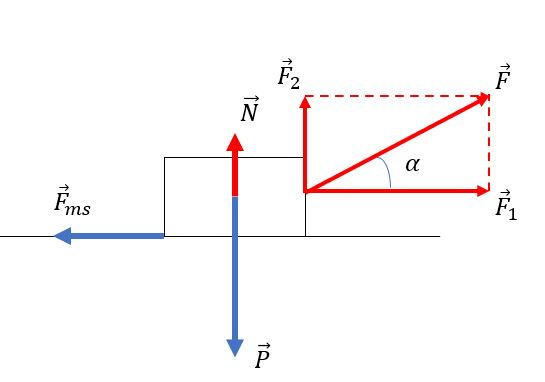
\includegraphics[scale=0.6]{../figs/VN10-PH-15-A-005-3-V2-02.JPG}
		\end{center} 
		 Áp dụng định luật II Newton 
			\begin{equation*}
				\vec{N}+\vec{P} + \vec{F}_{\text{ms}} + \vec{F} = m\vec{a}.
			\end{equation*}
		Chiếu lên O$y$:
			\begin{align*}
				N - P + F\sin \alpha  &= 0\\
				 \Rightarrow\quad N&=P - F\sin \alpha.	
			\end{align*}
		Chiếu lên O$x$:
			\begin{equation*}
				F\cos \alpha - F_{\text{ms}} = ma.
			\end{equation*}
		Độ lớn của lực kéo
			\begin{align*}
				F\cos \alpha - \mu(P - F\sin \alpha) &= ma\\
				\Rightarrow\quad F \cos \alpha - \mu (mg-F\sin \alpha) &= ma\\
				\Rightarrow\quad  F &=\dfrac{m(\mu g +a)}{\cos \alpha + \mu \sin \alpha}= \SI{3,87}{N}.
			\end{align*}
	}
	\viduii{3}{Một ô tô khối lượng 1 tấn, chuyển động trên mặt đường nằm ngang. Hệ số ma sát lăn giữa xe và mặt đường là 0,1. Tính lực kéo của động cơ ô tô trong mỗi trường hợp sau
		
		a) Ô tô chuyển động thẳng đều.
		
		b) Ô tô chuyển động nhanh dần đều với gia tốc $a = \SI{2}{m/s}^2$, lấy $g=\SI{10}{m/s^2}$.
	}
	{	\begin{center}
			\textbf{Hướng dẫn giải}
		\end{center}
		\begin{center}
			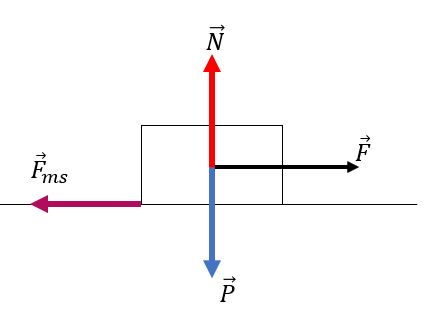
\includegraphics[scale=0.6]{../figs/VN10-PH-15-A-005-3-V2-03.JPG}
		\end{center} 
		Áp dụng định luật II Newton
			\begin{equation*}
				\vec{N}+\vec{P} + \vec{F}_{\text{ms}} + \vec{F} = m\vec{a}.
			\end{equation*}
		Chiếu lên O$y$:
			\begin{equation*}
				N=P = mg.
			\end{equation*}
		Chiếu lên O$x$:
			\begin{equation*}
				F-F_{\text{ms}} = ma \Rightarrow F = ma + F_{\text{ms}}
			\end{equation*}
		a) Khi ô tô chuyển động thẳng đều thì $a=0$ nên lực kéo của ô tô đúng bằng lực ma sát
		\begin{equation*}
			F=F_{\text{ms}} = \mu mg = \SI{1000}{N}.
		\end{equation*}
		b) Khi ô tô chuyển động nhanh dần đều với gia tốc $a = \SI{2}{m/s^2}$ 
		\begin{equation*}
			F= ma + F_{\text{ms}} = ma + \mu mg = m(a+ \mu g) = \SI{3000}{N}.
		\end{equation*}
		
	}
	
	\viduii{3}{Một xe lăn, khi được đẩy bằng lực $F = \SI{20}{N}$ nằm ngang thì xe chuyển động thẳng đều. Khi chất lên xe một kiện hàng khối lượng $\SI{20}{kg}$ thì phải chịu tác dụng lực $F = \SI{60}{N}$ nằm ngang xe mới chuyển động thẳng đều. Tính hệ số ma sát giữa xe và mặt dường.
	}
	{	\begin{center}
			\textbf{Hướng dẫn giải}
		\end{center}
		
		Chọn chiều dương là chiều chuyển động của xe.
		
		Khi chưa chất kiện hàng lên xe, xe chuyển động thằng đều nên:
		
		$$\vec P + \vec N + \vec F_\text{ms} + \vec F = \vec 0 \Rightarrow - F_\text{ms} + F =0 \Rightarrow F =F_\text{ms} = \mu mg\ (1).$$
		
		Khi đã chất kiện hàng lên xe, xe chuyển động thẳng đều nên:	
		
		$$\vec P' + \vec N' + \vec F'_\text{ms} + \vec F' = \vec 0 \Rightarrow - F'_\text{ms} + F' =0 \Rightarrow F' =F'_\text{ms} = \mu (m+m_\text{h})g\ (2).$$
		
		Từ (1) và (2) suy ra: 
		
		$$F' - F = \mu g m_\text{h} \Rightarrow \mu =\dfrac{F'-F}{gm_\text{h}} = \SI{0,2}{}.$$
		
		
	}
	
\end{dang}
